\section{INTRODUCTION}
Multi-robot systems belong to core robotics problems that have drawn significant attention in last few decades. The coordination of a mobile robot team during the exploration of an unknown area is a common problem encountered in many applications, such as search and rescue \cite{Murphy2004}, cleaning \cite{Endres}, \cite{Pinheiro2015}, warehousing \cite{Wurman2008}, or planetary exploration \cite{Mataric2001}, to name a few. Due to the fact that autonomous multi-robot systems are entering society domain and as such will interact with people on daily basis, development of efficient coordination algorithms becomes inevitable.

 Like in the human world, robots can be more effective when they work together. Moreover, a robot team can accomplish a predefined task much quicker than a single robot can \cite{Dias2000}. Another advantage of mobile robot teams arises from the possibility of merging overlapping sensor information, which in turn can help to compensate for sensor uncertainty \cite{Wurm2008}.
If is done properly, multi-robot coordination can lead to i) task accomplishment in the shortest possible time, ii) increased robustness, iii) higher map quality (in case of exploration task), and finally iv) the completion of tasks impossible for a single robot to perform \cite{Dias2006}.

\begin{figure}[t!]
    \centering
	\fbox{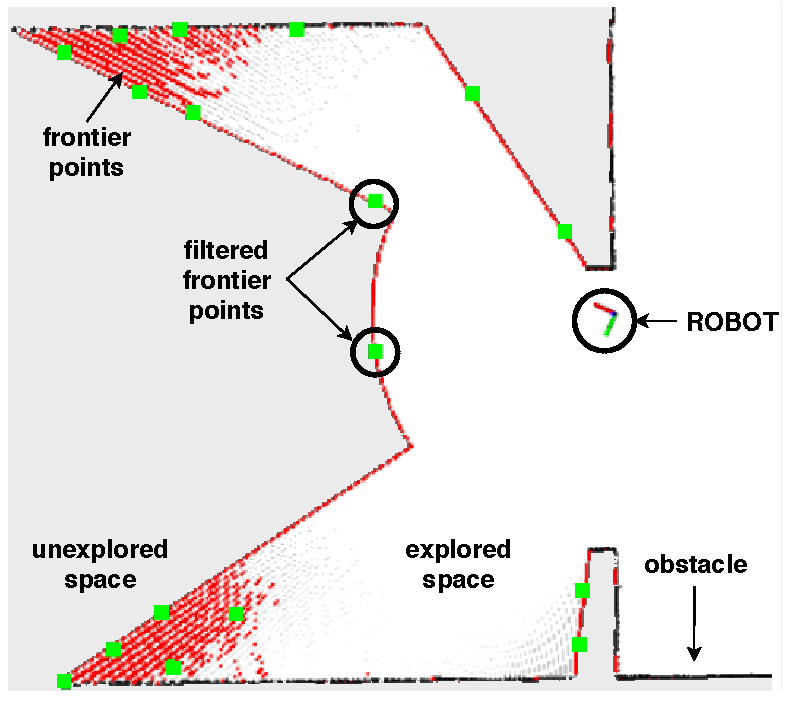
\includegraphics[width=0.85\columnwidth]{./Pictures/rviz_environment.pdf}}
	\caption {The description of the environment. A 2D map is represented with an occupancy grid that divides the map into cells: the white cells describe explored and grey cells unexplored space, while the black cells define obstacles. The frontier detector publishes frontier points (red) and the filter module publishes filtered frontier points (green).}
	\label{fig:environment}
\end{figure}


We consider the problem of autonomous multi-robot exploration and mapping using a fast dense frontier detector and a new decentralized exploration strategy. A result of frontier detection are points on the border of the explored and unexplored space in the environment - \textit{frontier points} shown in the Fig. \ref{fig:environment}. It is a dense set of frontier points, thus we use a filter to get a more manageable number of the frontier points. Since the main goal is to achieve faster exploration and better coordination among the mobile robots, our decentralized strategy ensures that the mobile robots become dispersed throughout the environment using a frontier occupancy function which takes into account current assigned points and position of all other mobile robots in exploration and mapping process. Every team member also calculates the cost and the utility of reaching all frontier points. Finally, the Hungarian algorithm \cite{Kuhn1955}, that attempts to find an optimal assignment solution (a target point for a mobile robot), is run by each mobile robot in parallel. It is assumed that communication among the mobile robots is modelled by a fully connected (complete) graph in order to avoid sub-optimal results as a consequence of information missing. 
If we consider connected communication graph but may not complete, then we need to think about a decentralized map generation, what is currently not our scope. An additional novelty of this work is the event based communication between mobile robots and minimum exchanging information about mobile robot positions and target points.  When a mobile robot is assigned to a frontier point for exploration, the algorithm for path planning and following navigates the mobile robot toward the target point. The process is over when the whole area is mapped.

The exploration and mapping strategy is implemented on multi-robot system using ROS framework. The strategy is compared to coordinated Burgard's Algorithm 1 \cite{Burgard2005}, which takes into account the costs of reaching a target and the utility of reaching that target. Whenever a target point is assigned to a specific robot team member, the utility of the unexplored area visible from this target position is reduced for the other team members. To emphasize, Burgard's and our utility functions have a different definitions, but lead to the same goal, minimum exploration time. The main difference between these two approaches is a target point assignment. This paper presents a new decentralized tagret point assignment process that enables all team members to be their own  \emph{leader} in contrast to the coordinated Burgard's approach, where the  \emph{leader} is a computer.

The rest of the paper is organised as follows. The exploration and mapping overview is presented in the next section. In Section III the exploration strategy is described. Simulation results are presented in Section IV, and in the final section a conclusion is given.
